\documentclass{article}
\usepackage[defaultfam,tabular,lining]{montserrat}
\usepackage[default]{lato}
\usepackage[T1]{fontenc}
\usepackage{sectsty}
\usepackage[HTML]{xcolor}
\usepackage{textcase}
\usepackage{multicol}
\usepackage{wrapfig}
\usepackage{graphicx}
\graphicspath{ {img/} }
\usepackage[a4paper, portrait, margin=1in]{geometry}
\allsectionsfont{\color[HTML]{008080}\fontfamily{Montserrat-TOsF}\selectfont\MakeTextUppercase}
%\renewcommand*\oldstylenums[1]{{\fontfamily{Montserrat-TOsF}\selectfont #1}}
\begin{document}

\title{Curriculum Vitae}
\author{Simon Fish}

%\maketitle
\begin{wrapfigure}{r}{0.25\textwidth}
			           \centering
				       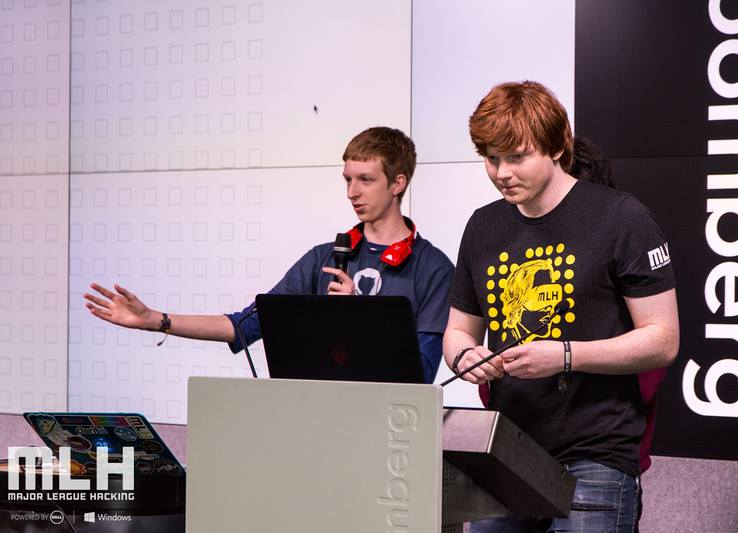
\includegraphics[width=0.25\textwidth]{profile}
		       \end{wrapfigure}

   \begin{center}
	         \color[HTML]{008080}\fontfamily{Montserrat-TOsF}\selectfont\MakeTextUppercase\Large\textbf{SIMON FISH}\\
		       \small\textit{simon.fish | si@mon.fish | 07852 406718 | 42 Tolethorpe Close, Oakham, Rutland LE15 6GF}
		       		       %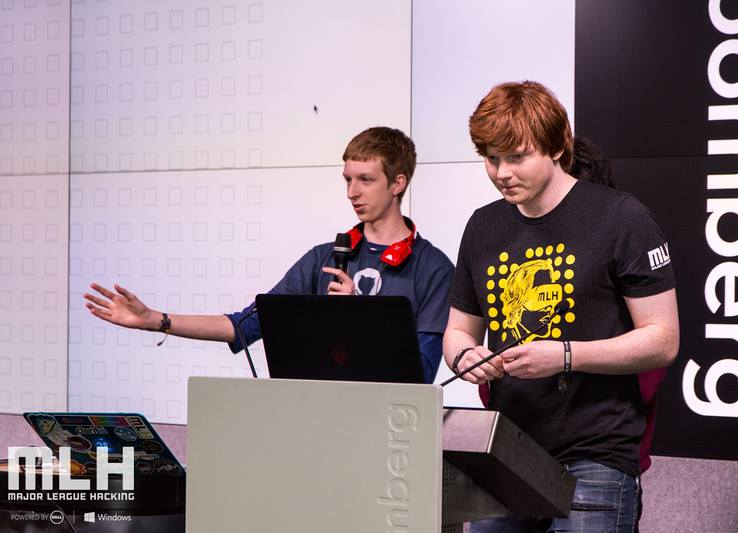
\includegraphics[width=3cm]{profile}
		          \end{center}

\section*{Profile}
A diligent and efficient worker who is always willing to learn. I enjoy using logic to
overcome challenges. My technical ability allows me to clear tasks efficiently,
while also ensuring that the end product is of high quality. My logical mind
ensures that I can quickly reach a conclusion, and equally, creativity also
contributes to my success. I have developed strong determination and a highly
positive outlook.

\section*{Education}
\subsection*{University of Sheffield | 2016-present}
\subsubsection*{Computer Science with a Year in Industry, BSc}
\paragraph{First Year}
My first year consists of the following modules:
\begin{multicols}{2}
\begin{itemize}
  \item Intro to Software Engineering
  \item Foundations of Computer Science
  \item Java Programming
  \item Machines and Intelligence
  \item Devices and Networks
  \item Web \& Internet Technology
  \item Algorithms \& Data Structures
\end{itemize}
\end{multicols}
\paragraph{Other Experience}
\begin{itemize}
	\item Programming Languages
	\begin{multicols}{2}
	\begin{itemize}
	\item Python
	\item Ruby
	\item Java
	\item Shoes toolkit for Ruby
	\item Swing/AWT for Java
	\item HTML
	\item CSS
	\item JavaScript
	\item jQuery
	\item Bootstrap
	\end{itemize}
	\end{multicols}
	\end{itemize}
\begin{itemize}
	\item Operating Systems 
		\begin{itemize}
			\item Windows (98, XP, 8, 8.1, 10)
			\item Linux (Ubuntu KDE, Fedora, Debian, Openbox, i3)
		\end{itemize}
\end{itemize}
\paragraph{A Selection of Completed Projects}
\begin{itemize}
  \item Website for children's online game company in core HTML/CSS (77\%) 
  \item Customisable remake of \textit{Flood-It!} in Ruby (80\%) 
  \item Connect 4 game operable by both CLI and GUI in Java
  \item Personal website, simon.fish, using Bootstrap
  \item Experimental GUI in Shoes, a Ruby toolkit, that writes to a .json file
  \item Text adventure game engine controlled using Amazon Alexa-capable devices, with live web statistics (co-developed with a team at GreatUniHack 2016)
  \item Script that uses APIs to retrieve chronological data from GitHub and Twitter (personal reimplementation of an idea from HackNotts 2016)
  \item Online multiplayer in-browser \textit{Bomberman} clone (co-developed with a team at MLH Prime EU Regional)
\end{itemize}
\subsection*{Brooke Weston Academy | 2014-2016}
\begin{itemize}
	\item Dist\* grade in Cambridge TEC Level 3 IT, A grade in A2 Maths, B grade in AS German and C grade in A2 Further Maths
\end{itemize}
\subsection*{Catmose College | 2011-2014}
\begin{itemize}
	\item 4 A\* grades, 3 A grades and 2 B grades, plus BTEC Level 2 in Music at Dist\* 
\end{itemize}
\section*{Work Experience}
\subsection*{Pera Technology | 2013-2014}
\begin{itemize}
\item Applied and improved programming skills in SQL and Python.
\item Returned for six weeks of paid work following work experience, being the first to do so in the Central Management division's recent history
\item Crafted an inexpensive surveillance solution for use in the company's laboratories
\item Took part in the pitching process for a confidential project
\end{itemize}
\subsection*{Central England Co-operative | 2014-2016}
\begin{itemize}
\item Worked primarily in grocery and on checkouts, requiring both physical diligence and situational communication
\item Heavily increased confidence in social situations in this role
\item Worked in positions of high responsibility, managing age-restricted goods such as petrol and tobacco, and was able to lead the team on several occasions
\end{itemize}
\section*{Accolades}
\begin{itemize}
\item Received a rare monetary reward through Pera Technology's BRAVO! Scheme
\item Received a monetary reward and Academic Scholarship from the Principal for my contributions as Subject Ambassador for Computer Science
\end{itemize}
\section*{Personal Interests}
\begin{itemize}
\item Enthusiasm for listening to and composing music digitally, requiring DAWs such as FL Studio and Logic Express 9.
\item Engaging with the news and current affairs
\item Writing and creating original content
\item Building and customising PCs
\item Hosting and improving my personal website
\item Building projects with others at hackathon events
\end{itemize}
\end{document}
